%
\section{Templates for QtCreator}\label{sec:templateqtcreator}
%
The SailfishOS SDK comes with a template for a new SailfishOS Qt Quick Application project.
%
\begin{figure}[H]
  \centering
  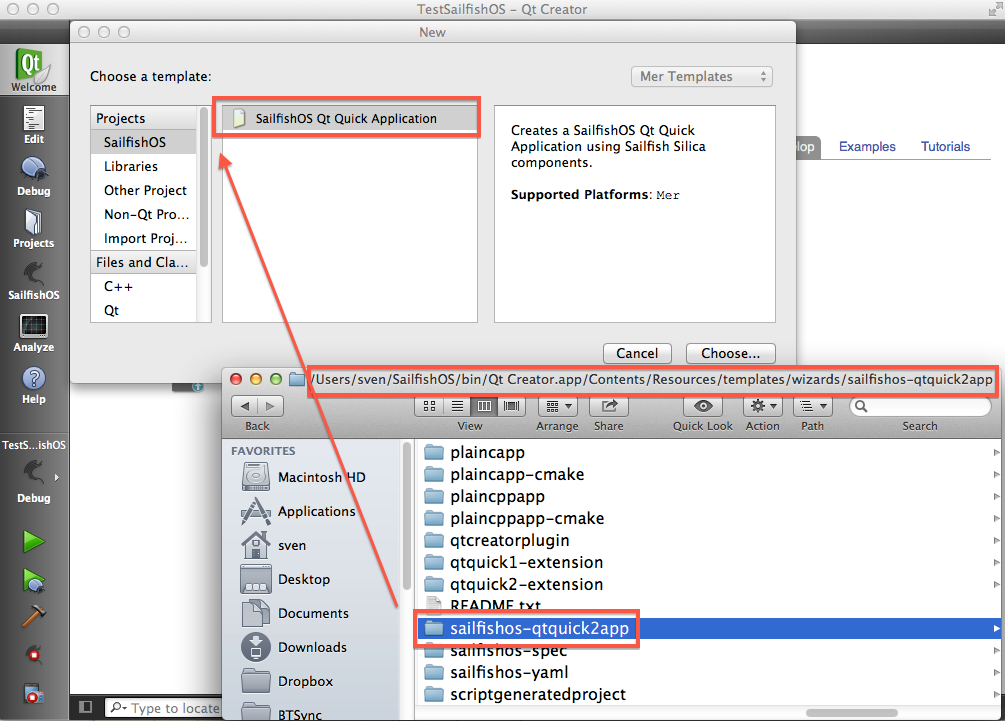
\includegraphics[scale=0.4]{../media/gfx/QtCreator/newprojecttemplate1.png} 
  \caption{Template for a new SailfishOS Qt Quick Application.}
  \label{fig:newprojecttemplate1}
\end{figure}
%
%
\subsection{OSX}
%
On OSX those templates are stored inside the QtCreator bundle\footnote{Bundles are just directories that end on .app are shown as one object in the finder.} on OSX. To access them you need to show the package content
%
\begin{figure}[H]
  \centering
  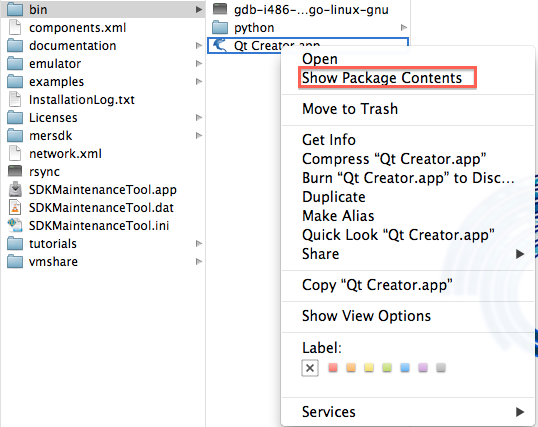
\includegraphics[scale=0.6]{../media/gfx/QtCreator/templates01-01.png} 
  \caption{OSX, show package content.}
  \label{fig:template01-01}
\end{figure}
%
or use your terminal.
%
\begin{lstlisting}[language=bash]
ls ~/SailfishOS/bin/Qt\ Creator.app/Contents/Resources/templates/wizards
\end{lstlisting}
%
\subsection{Linux}
%
TODO
%
%
\subsection{Windows}
TODO
%
%
%
\subsection{Generic}
TODO
%
You can change those given templates there or create new ones.

Just make sure that you don't use the names \verb,, \verb,obj,, \verb,moc,, \verb,ui, or \verb,rcc, inside your template. These are going to be used to store the compile results and temporaries if you compile a SailfishOS program.

Updates of the SDK may delete changed or new templates, you might want to create a backup in a safe place and restore afterwards.
There are three categories of files.
\begin{enumerate}
\item \verb,wizard.xml, contains information which files end up where in your new created project, what icon is shown in QtCreator as a symbol for this project type and the information you are asked while you create the project, like e.g. project name, version number and description.
\item an icon file that represents the project type in QtCreator. That is \emph{not} the icon of your future application. So far the template for new SailfishOS Qt Quick Application project has no specific icon. 
\item template files that end up in your new created project, all \verb,.pro,,\verb,.h,,\verb,.cpp,,\verb,.qml, and \verb,.png, files. While those files are copied, some of the information\footnote{Like the filename itself or details inside a file, e.g. the TARGET in the .pro file.} can be transformed and that is also defined in the \verb,wizard.xml, file.
\end{enumerate}
%
TODO more details.
%
Much more information of the format of the \verb,wizard.xml, file can be found in \cite{qt07}.
%